\section{Data and Monte Carlo Samples}
\label{sec:DataAndMC}

The data sample we use in this measurement was recorded by the CMS experiment in~2012 in LHC $pp$ collisions at $\sqrt{s}=$8~TeV. Integrated luminosity of the dataset is $L=$19.6~fb$^{-1}$. To select $W\gamma$ events, we use data collected by single muon and single electron triggers. The single muon trigger requires that in each event there is at least one reconstructed isolated muon with $P_T^{\mu}>$24~GeV and $|\eta|<$2.1. The single electron trigger requires at least one reconstructed electron with $P_T^{e}>$27~GeV which also passes a certain set of identification requirements, including isolation. Such trigger choice maximize our chances to select $W\gamma$ events out of dominant multijets events.

In addition to $W\gamma$-selected data sample, we also prepare $Z\gamma$-selected data sample which is used for the background estimation (Ch.~\ref{sec:BackgroundSubtraction}) and for cross checking purpose (App.~\ref{sec:ZgCheck}). To select $Z\gamma$ events, we use double muon and double electron triggers. The double muon trigger requires a presence of at least two reconstructed muons with $P_T^{\mu}>$17~GeV and $P_T^{\mu}>$8~GeV per event. The double electron trigger requires a presence of at least two reconstructed electrons with $P_T^{e}>$17~GeV and $P_T^{e}>$8~GeV which also satisfy several other criteria of electron's quality.

%_HLT_Mu17_Mu8_v
%_HLT_Ele17_Ele8_v, many other conditions

 % are used as the signal samples while double muon and double electron datasets are used for data-driven background estimation. 

%The data is collected by single electron ($p_T>27$~GeV, WP 80) 
%and single muon ($p_T>24$~GeV, $|\eta|<2.1$) triggers

% Only runs and luminosity sections certified by CMS are considered in the measurement, 
% which means that good functioning of all CMS sub-detectors is required.

%THE IDEAS FROM THIS PARAGRAPH NEED TO BE REPACKAGED
All simulated samples (often referred as Monte Carlo or MC samples) used in this measurement are generated with MadGraph~\cite{ref_MadGraph} and reconstructed centrally by the CMS simulation team. Information regarding MC samples used for our measurement is given in Tab.~\ref{tab:mc_bkg_samples} alongside with the corresponding cross sections at~8~TeV. All cross sections are calculated with kinematic restrictions matching to the kinematic restrictions of the samples. 

When we select $W\gamma$ events, certain number of events from other processes pass the selection criteria too. Tab.~\ref{tab:mc_bkg_samples} contains all sources that significantly contribute to the selected sample. $W\gamma \rightarrow l\nu\gamma$ contains $W\gamma \rightarrow \mu\nu\gamma$ and $W\gamma \rightarrow e\nu\gamma$ which are our signal samples and $W\gamma \rightarrow \tau\nu\gamma$ which is a background for both channels. The other samples listed in Tab.~\ref{tab:mc_bkg_samples} are background samples. They are used for the background estimation and cross checking as explained in detail in the remainder of the chapter.


\begin{table}[h]
  \small
  \begin{center}
    \caption{Summary of simulated samples used in the measurement.}
    \begin{tabular}{|l|l|l|}
      \hline
      Process                              & Type & $\sigma$, pb  \\ \hline
      $W\gamma \rightarrow l\nu\gamma$     & signal & 554   \\ \hline %(NLO MCFM)
      $W$+jets$ \rightarrow l\nu $+jets   & background & 36257  \\ \hline %(NNLO FEWZ)
      DY+jets$ \rightarrow ll $+jets     & background & 3504  \\ \hline %(NNLO FEWZ)
      $t\bar{t}$+jets$\rightarrow 1l$+X    & background & 99    \\ \hline %(NNLO)
      $t\bar{t}$+jets$\rightarrow 2l$+X    & background & 24    \\ \hline
%      $t\bar{t}\gamma$                     & background & 1    \\ \hline
      $Z\gamma \rightarrow ll\gamma$       & background & 172   \\ \hline
    \end{tabular}
    \label{tab:mc_bkg_samples}
  \end{center}
\end{table} 

% QUOTE: WJets, DYjets:
%Signal and background processes are generated with various state-of-the-art generators and passed through detector simulation based on GEANT 4 [14] description of CMS. Each simulated sample is normalized to the integrated luminosity of the data sample. The simulated events are required to pass an emulation of the trigger requirements applied to the data. Trigger efficiencies in the simulation are corrected for differences with respect to the data.  Simulations also include additional collisions in the same or adjacent bunch crossings (pileup, PU). To model PU, minimum-bias events generated with PYTHIA 6 using the Z2* tune [15] are superimposed on the simulated events, matching the multiplicity of PU collisions observed in data, which has an average value of approximately 21. The W+jets signal process is simulated with the matrix element (ME) generator MADGRAPH 5.1.1 [1] interfaced with PYTHIA 6.426 using the Z2* tune for parton showering and hadronization.  This sample of events, denoted MADGRAPH 5 + PYTHIA 6 (denoted as MG5+PY6 in the figure  legends),  is  produced  with  the  CTEQ6L1  parton  distribution  function  (PDF)  set   3 and  is  normalized  to  the  inclusive  NNLO  cross  section  calculated  with FEWZ 3.1  [17].   The MADGRAPH5+PYTHIA 6 calculation includes the production of up to four partons at LO. The jets from matrix elements are matched to parton showers following the kT-jet MLM prescription [18], where partons are clustered using the kT algorithm [19] with a distance parameter of 1. The merging of parton showers and matrix elements with the MLM scheme uses a matching scale of 20 GeV.  The factorization and renormalization scales for the 2 →2 hard process in the event are chosen to be the transverse mass of the W boson produced in the central process. The kT computed for each QCD emission vertex is used as renormalization scale for the calculationof the strong coupling constantαS of that vertex. Background processes include tt, single top quark, Z/γ∗+jets, diboson (ZZ/WZ/WW) + jets, and QCD multijet production.  Their contributions, with the exception of QCD multijet pro-duction, are estimated from simulation. The simulated samples of tt and Z/γ∗+jets events are generated with MADGRAPH version 5.1.1; the single top quark samples (s-, t-, and tW-channel production) are generated with POWHEG version 1 [20–23]; and the diboson samples (WW, WZ, or ZZ) are generated with PYTHIA6.424 using the Z2∗tune. The simulations with MADGRAPH and PYTHIA use the CTEQ6L1 PDFs, and the simulations with POWHEG use the CTEQ6M PDFs. The Z/γ∗+jets sample is normalized to the NNLO inclusive cross section calculated with FEWZ 3.1 [17]. Single top quark and diboson samples are normalized to NLO inclusive cross sections calculated with MCFM [24–27]. The tt contribution is normalized to the predicted cross section at NNLO with next-to-next-to-leading-logarithm accuracy [28]. When comparing the measurements with the theoretical prediction, other event generators are used for the W+jets process. Those generators, which are not used for the measurement itself, are described in Section

%Signal and background processes are generated and passed through detector simulation based on GEANT~4 description of CMS. Each simulated sample is normalized to the integrated luminosity of the data sample. 

The W+jets process is simulated with the matrix element (ME) generator MADGRAPH~5.1.1 interfaced with PYTHIA~6.426 using the~Z2* tune for parton showering and hadronization.  This sample of events is produced with the CTEQ6L1 parton distribution function (PDF) set and is  normalized  to  the  inclusive  NNLO  cross  section  calculated  with FEWZ~3.1.   The MADGRAPH 5 + PYTHIA 6 calculation includes the production of up to four partons at LO. The jets from matrix elements are matched to parton showers following the $k_T$-jet MLM prescription, where partons are clustered using the $k_$ algorithm with a distance parameter of 1. The merging of parton showers and matrix elements with the MLM scheme uses a matching scale of~20~GeV.  The factorization and renormalization scales for the~$2\rightarrow 2$ hard process in the event are chosen to be the transverse mass of the W boson produced in the central process. The $k_T$ computed for each QCD emission vertex is used as renormalization scale for the calculation of the strong coupling constant $\alpha_S$ of that vertex. 

Another significant background process for $W\gamma$ is DY+jets where DY is a notation for the Drell Yan process which is $pp\rightarrow\Z/\gamma\rightarrow ll$. The simulated sample of DY+jets events is generated with MADGRAPH version~5.1.1. This simulation uses the CTEQ6L1 PDFs. The DY+jets sample is normalized to the NNLO inclusive cross section calculated with FEWZ~3.1. The requirement on the invariant mass of the final state lepton pair is $M_{ll}>$50~GeV. Samples $W$+jets and DY+jets are prepared in a way they do not overlap with $W\gamma$ and $Z\gamma$ samples.

All MC samples are normalized to the luminosity of the dataset $L=19.6~$pb$^{-1}$. To perform the normalization, appropriate weights are applied to each event in each MC sample. Such weighted MC samples are often used for various MC estimates and for plotting histograms for data vs MC comparisons.

The NLO cross section of $W\gamma$ was calculated with the MCFM in the same phase space for which the $W\gamma$ sample was generated. The NNLO contribution is estimated to be~19\%-26\% of the NLO value~\cite{ref_theory_NNLO}. We use an NLO cross section value, and the NNLO estimate is used as an systematic uncertainty of the normalization of the $W\gamma$ sample when it is applicable. 

The uncertainty on normalization of the $Z\gamma$ sample gives a significant contribution to the uncertainty of a the measurement because $Z\gamma$ MC sample is used to estimate the most significant background (Ch.~\ref{sec:BackgroundSubtraction_jtog}). MCFM provides a value of the cross section with uncertainty of 20\%. To minimize the uncertainty, we use a cross section of $Z\gamma$ measured at~8~TeV by CMS~\cite{ref_Zg8TeV} and recalculated it for the phase space of the generated $Z\gamma$ MC sample. 

The $Z\gamma$ cross section of $\sigma = $2073$ \pm$ 95 $\pm$11$ \pm $53~fb has been quoted in the phase space described in~\cite{ref_Zg8TeV}. To determine the measured cross section in the generator phase space, the following formula was used:
\begin{equation}
\sigma_{ps1} = \sigma_{ps2}^{meas.} \cdot \frac{N_{ps1}^{MC}}{N_{ps2}^{MC}},
\end{equation}
\noindent{where $\sigma_{ps2}^{meas.}$ is the~8~TeV cross section measured by CMS, $N_{ps1}^{MC}$ and $N_{ps2}^{MC}$ are numbers of events in the full phase space of $Z\gamma$ MC samples and in the phase space corresponding to the measured cross section  $\sigma_{ps2}^{meas.}$, $\sigma_{ps1}$ is the resulting cross section of the $Z\gamma$ sample in its full phase space. }

The resulting $Z\gamma$ cross section is found to be~$172$~pb. Uncertainties on normalizations of other samples do not contribute significantly to the uncertainty of the measurement, therefore, we use MCFM values for them.

%HOW ZGamma Cross section was mapped to a different phase space (from AN):
%The cross section of Zg was computed using as inputs MCFM cross section values as well as the precise CMS measurement~\cite{Zg8TeV} using the following procedure. The Z$\gamma$ cross section of $\sigma = 2073 \pm 95 \pm \11 \pm \53$ fb has been quoted in the phase space described in ~\cite{Zg8TeV}. To determine the measured cross section in the generator phase space, the following formula was used:\\
%$\sigma_{narrow phase space}^{meas.}/\sigma_{wide phase space}^{meas.} = \sigma_{narrow phase space}^{MCFM}/\sigma_{wide phase space}^{MCFM}$.\\
%The $\sigma_{narrow phase space}^{MCFM}$ was determined by computing how many events are falling into the narrow phase space and scaling it to $\sigma_{wide phase space}^{MCFM}$=159.12 pb. The $\sigma_{narrow phase space}^{MCFM}$ was found to be 1933 fb and 1911 fb for the muon and electron channels respectively and the average of 1922 fb was used in the formula. The $\sigma_{wide phase space}^{meas.}$ was found to be 171.62 pb.

%EXPLAIN THE NEED FOR REQEIGHTING
At the instantaneous luminosities of LHC in~2012, as a rule, multiple $pp$ interactions occurred per bunch crossing. Multiple interactions are also simulated in the MC samples. However, MC samples are usually produced before data collection is finished, and in the end have to be reweighted so that the distribution of the number of interactions (pileup or PU) in a simulated sample matches the data. The PU weights are assigned on each event in each MC sample to make the PU distribution in MC accurately describe PU in data.

%EXPLAIN THE PROCEDURE OF REWEIGHTING (last sentence in previous paragraph)


%EXPLAIN THE VALIDATION OF REWEIGHTING
To validate the procedure of the PU reweighting, we check the agreement between data and MC in the distribution of the number of vertices in $Z\gamma\rightarrow\mu\mu\gamma$-selected datasets (Fig.~\ref{fig:DATAvsMC_nVtx}). We choose the $Z\gamma$ selected dataset instead of the $W\gamma$-selected dataset because the sample composition for $Z\gamma$ selection is understood better and normalizations of the MC samples that pass $Z\gamma$ selection are known better. The $Z\gamma$ selection is explained in Ch.~\ref{sec:AN_Selection} alongside with the $W\gamma$ selection.

\begin{figure}[htb]
  \begin{center}
   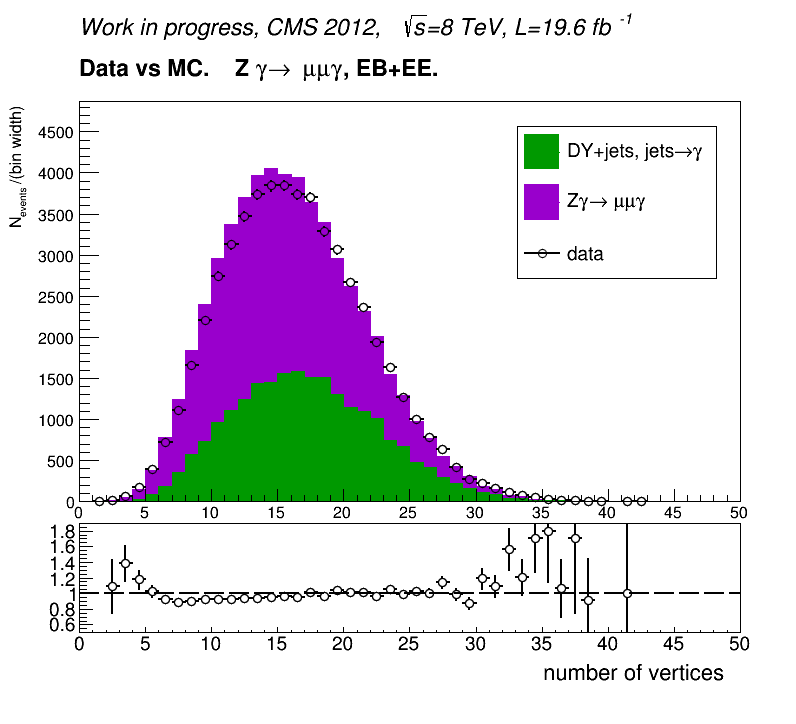
\includegraphics[width=0.45\textwidth]{../figs/figs_v11/MUON_ZGamma/PrepareYields/c_TotalDATAvsMC_EtaCommon__nVtx_noPU.png}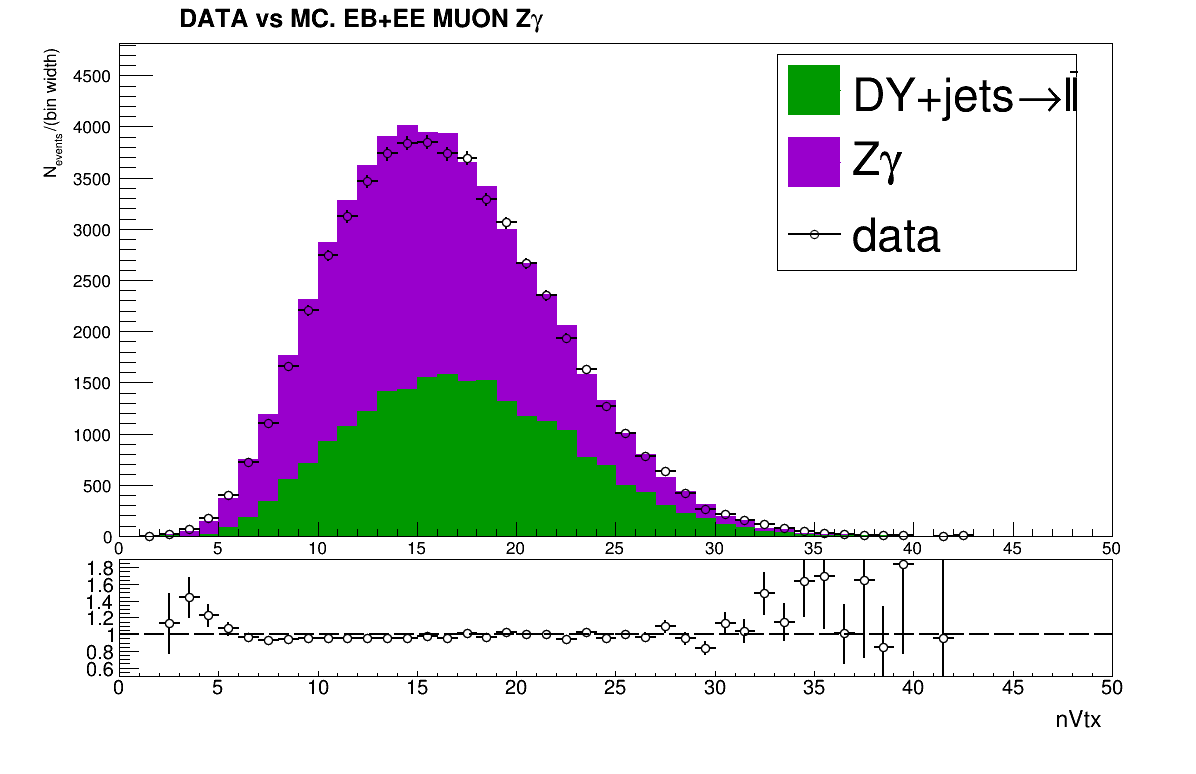
\includegraphics[width=0.45\textwidth]{../figs/figs_v11/MUON_ZGamma/PrepareYields/c_TotalDATAvsMC_EtaCommon__nVtx.png}
  \caption{Number of vertices of $Z\gamma$ candidates in the muon channel. Data vs MC. Left: no PU reweighting applied, right: PU reweighting applied. Ratio plot in the bottom shows data yields divided over total MC yields. EB+EE means that events with a final state photon reconstructed in the ECal barrel as well as  events with a final state photon reconstructed in the ECal endcap are shown on the plots.}
  \label{fig:DATAvsMC_nVtx}
  \end{center}
\end{figure}
